\vspace{-30pt}
\chapter{Planning EM}
\section{Introduction}
\begin{wrapfigure}{r}{0.35\textwidth}
\vspace{-50pt}
  \begin{center}
    \begin{tabular}{c}
\includegraphics[scale=0.35]{./Figure/Planning.EM/UnitCell.png}\tabularnewline
(a)\tabularnewline
\end{tabular}
\caption{\footnotesize (a) - Unit Cell modelled in HFSS}
  \end{center}
  
\end{wrapfigure}
As stated in the previous section, improving the quality of service
is crucial in an urban environment. Thus follows the reason behind
the following work: planning a SEE using a single or combined EMSs
to improve the quality of service in specific areas. To achieve the
stated goal, the EMSs are going to be shaped using a Unit Cell adapted
for every chosen spot. 
In the following discourse, various EMSs are going to be strategically
shaped and placed to fit the SEE that needs improving. 
All of the following described steps are going to be applied for every
RoI in the same way, adjusting just the quantity of EMSs and the characteristics
for every EMS.
\vspace{10pt}
\section{Scenario}
\subsection{Parameters}
\begin{minipage}{0.45\textwidth}
\begin{itemize}
\footnotesize
\item Dimensions of scenario: $D_{x}=D_{y}=1500[m]$
\item Resolution: $\Delta_{x}=\Delta_{y}=5[m]$
\item BTS Position: $r_{\Psi}=(850,850,30)[m]$
\item BTS Power: $P_{TX}=20[W]$
\item BTS Sectors: $3$
\item BTS Azimuth Angular Extension: $\Delta\phi=120[deg]$
\item Spacing: $\lambda/2$
\end{itemize}
\end{minipage}
\begin{minipage}{0.4\textwidth}
%\hspace{-50pt}
\begin{figure}[H]
\begin{tabular}{c}
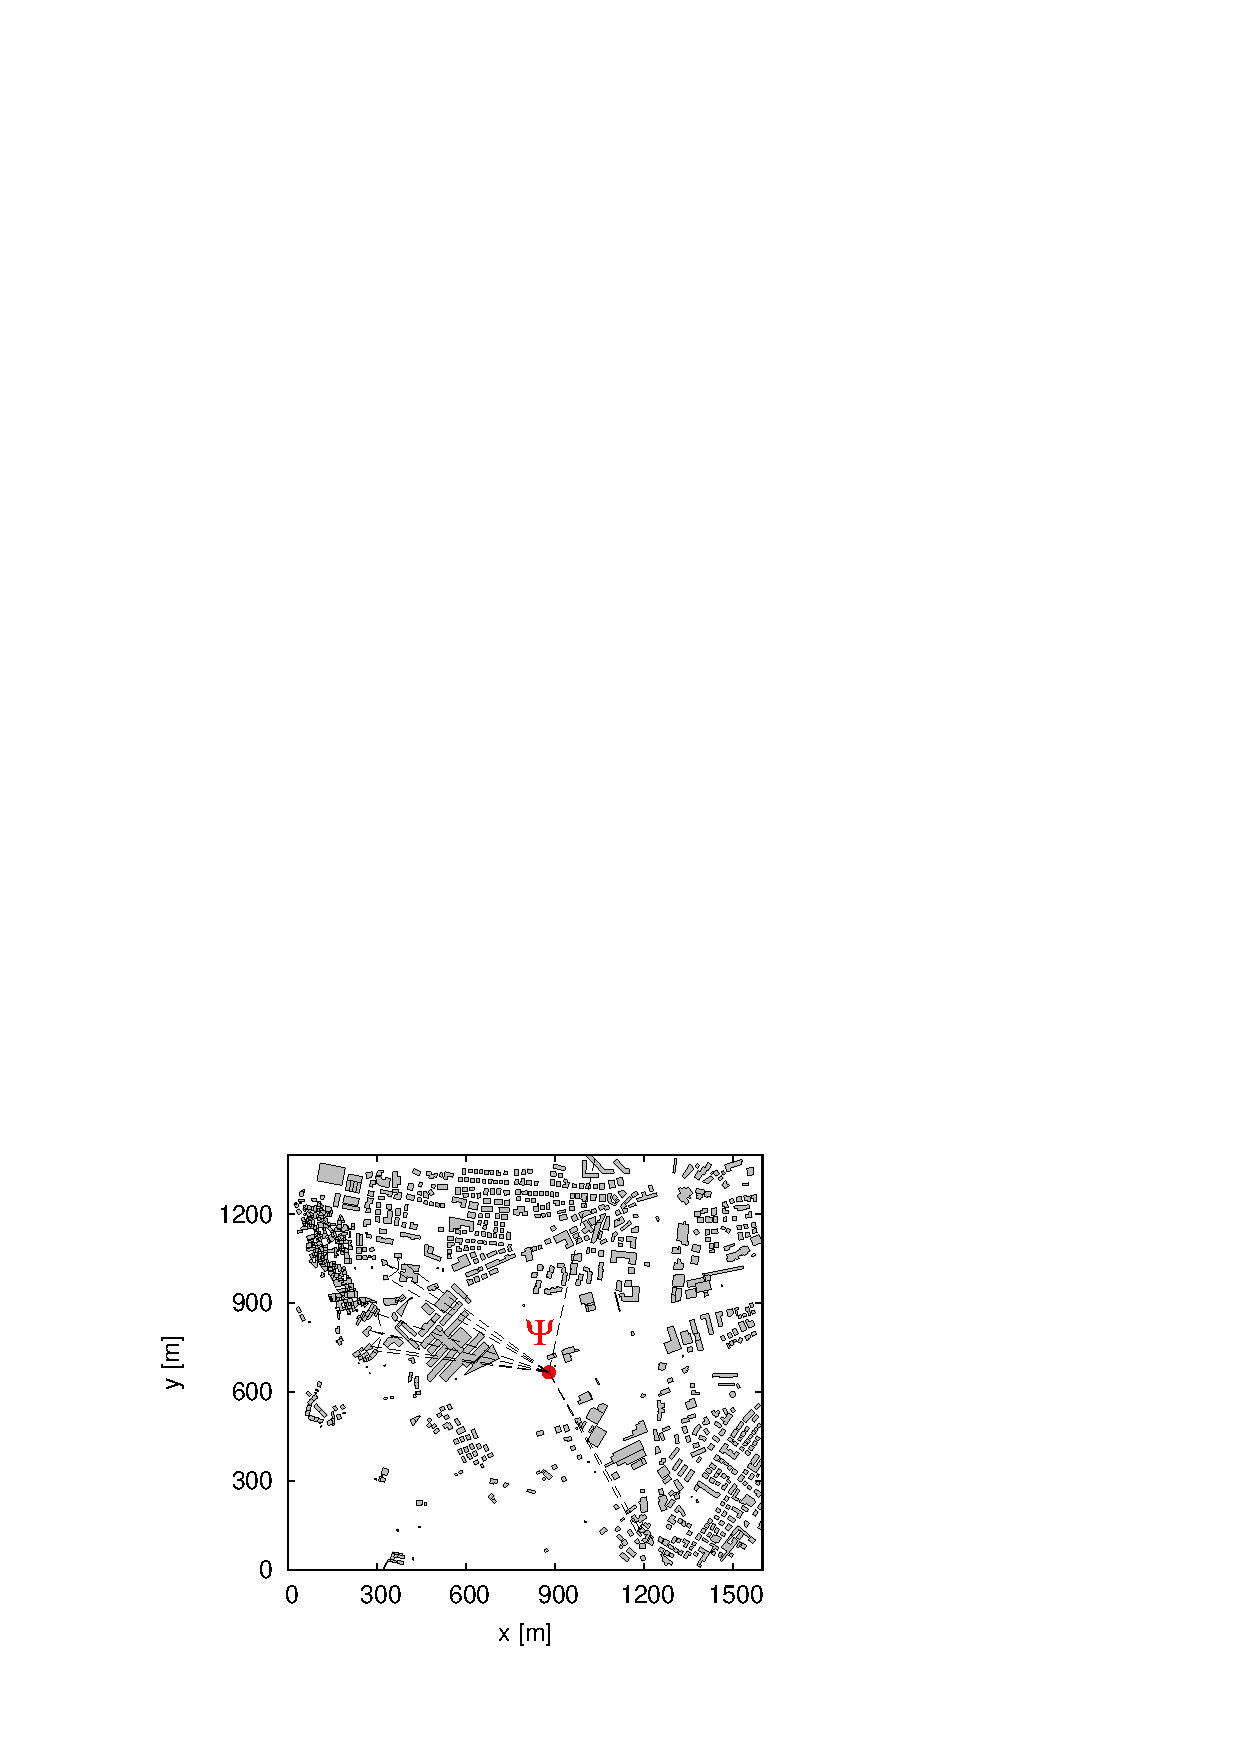
\includegraphics[scale=0.12]{./Figure/Planning.EM/Fig.Scenario.BTS.jpg}
\tabularnewline
\emph{(a)}\tabularnewline
\end{tabular}
\end{figure}
\end{minipage}
\vspace{-10pt}
\subsubsection{Scenery Presentation}
The first step is to define and model the scenario.

\begin{figure}[H]
\begin{center}\begin{tabular}{cc}
\includegraphics[scale=0.075]{./Figure/Planning.EM/Fig.Scenario.Rovereto.OSM.jpg}&
\includegraphics[scale=0.075]{./Figure/Planning.EM/Fig.Scenario.Rovereto.GM.jpg}\tabularnewline
\emph{(b)}&\emph{(c)}\tabularnewline
\end{tabular}\end{center}

\vspace{-10pt}
\caption{\footnotesize \emph{(a)} Scenario in WinProp \emph{- (b)} Scenario in OpenStreetMap
\emph{- (c)} Scenario in GoogleMaps}
\end{figure}
\vspace{-10pt}
\subsection{Power and Threshold}

Analyzing the radiaton pattern and thresholded pattern is needed to
find weak spots inside the scenario.

%
\begin{figure}[H]
\begin{center}\begin{tabular}{cc}
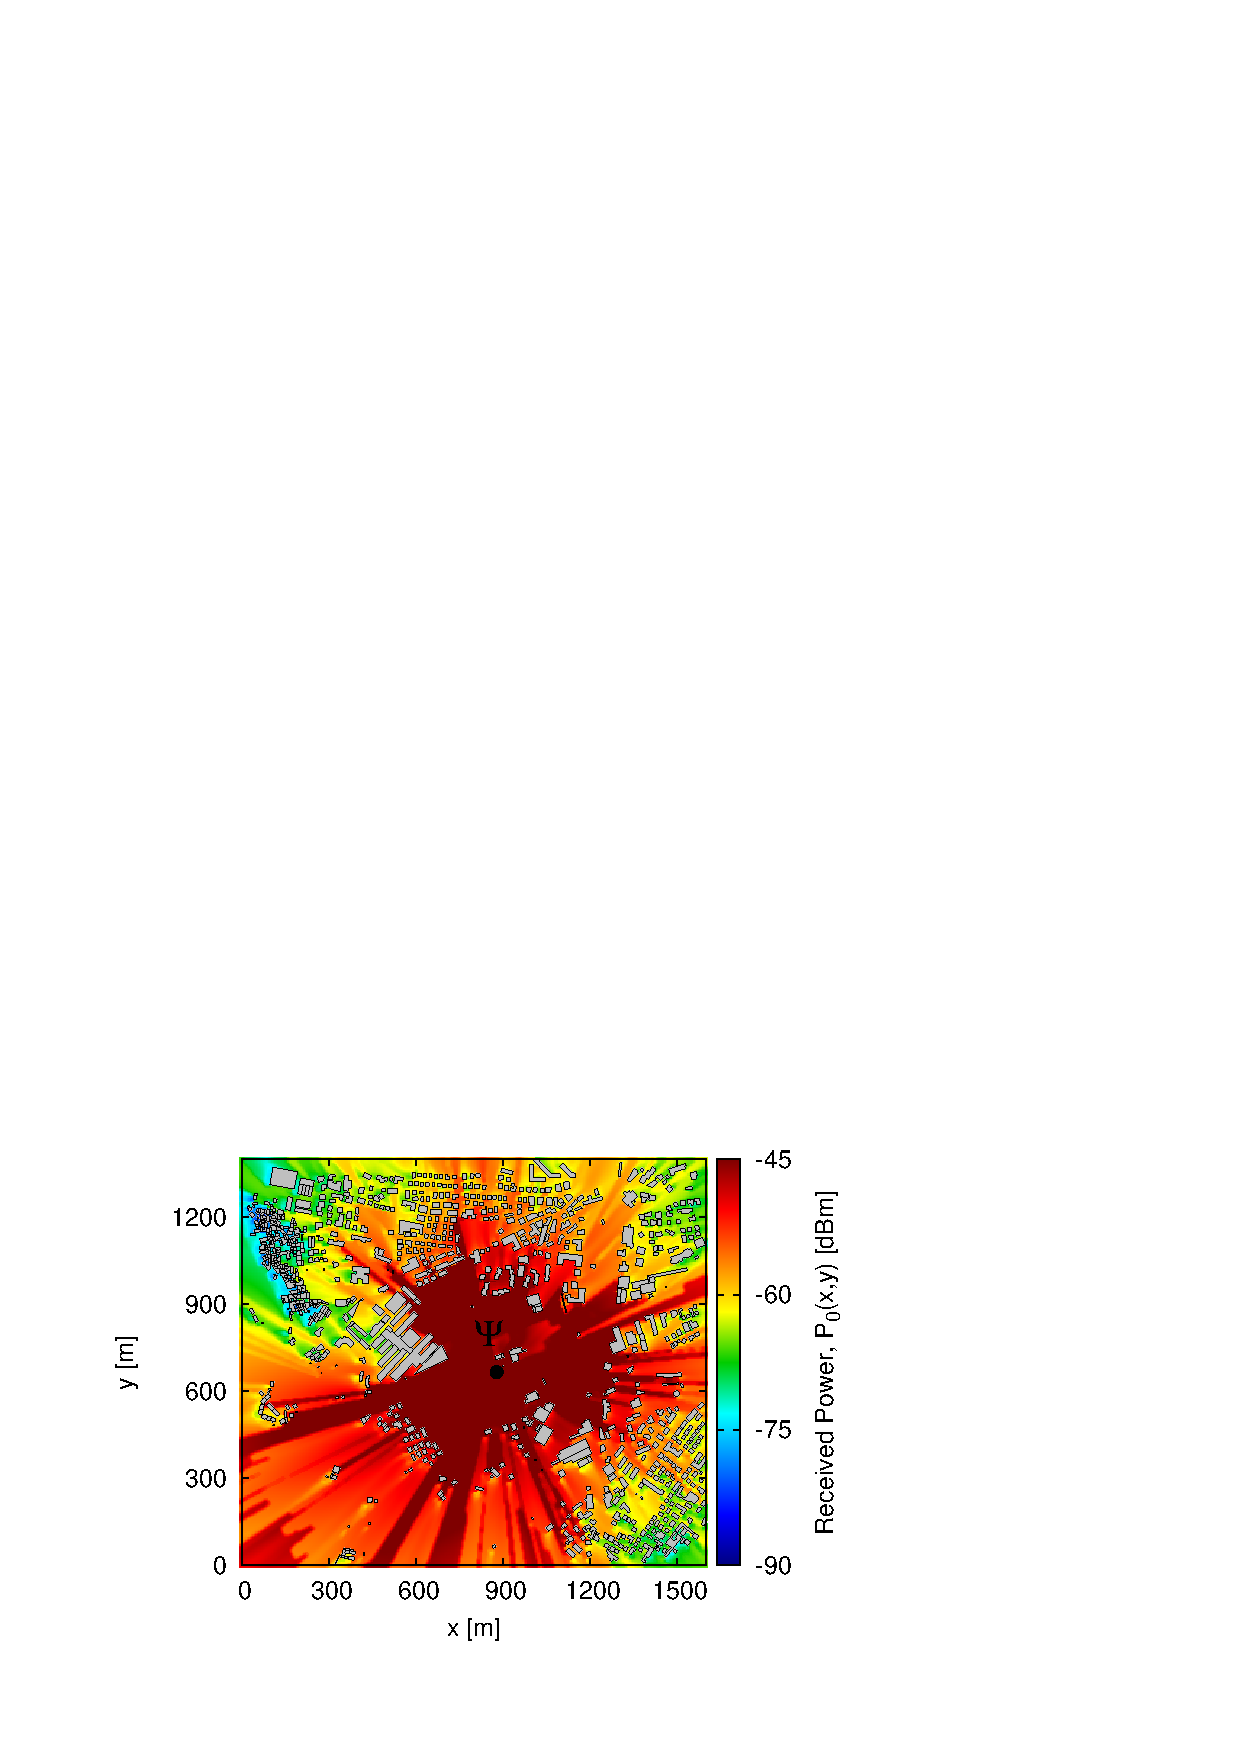
\includegraphics[scale=0.12]{./Figure/Planning.EM/Fig.Received.Power.Reference.jpg}&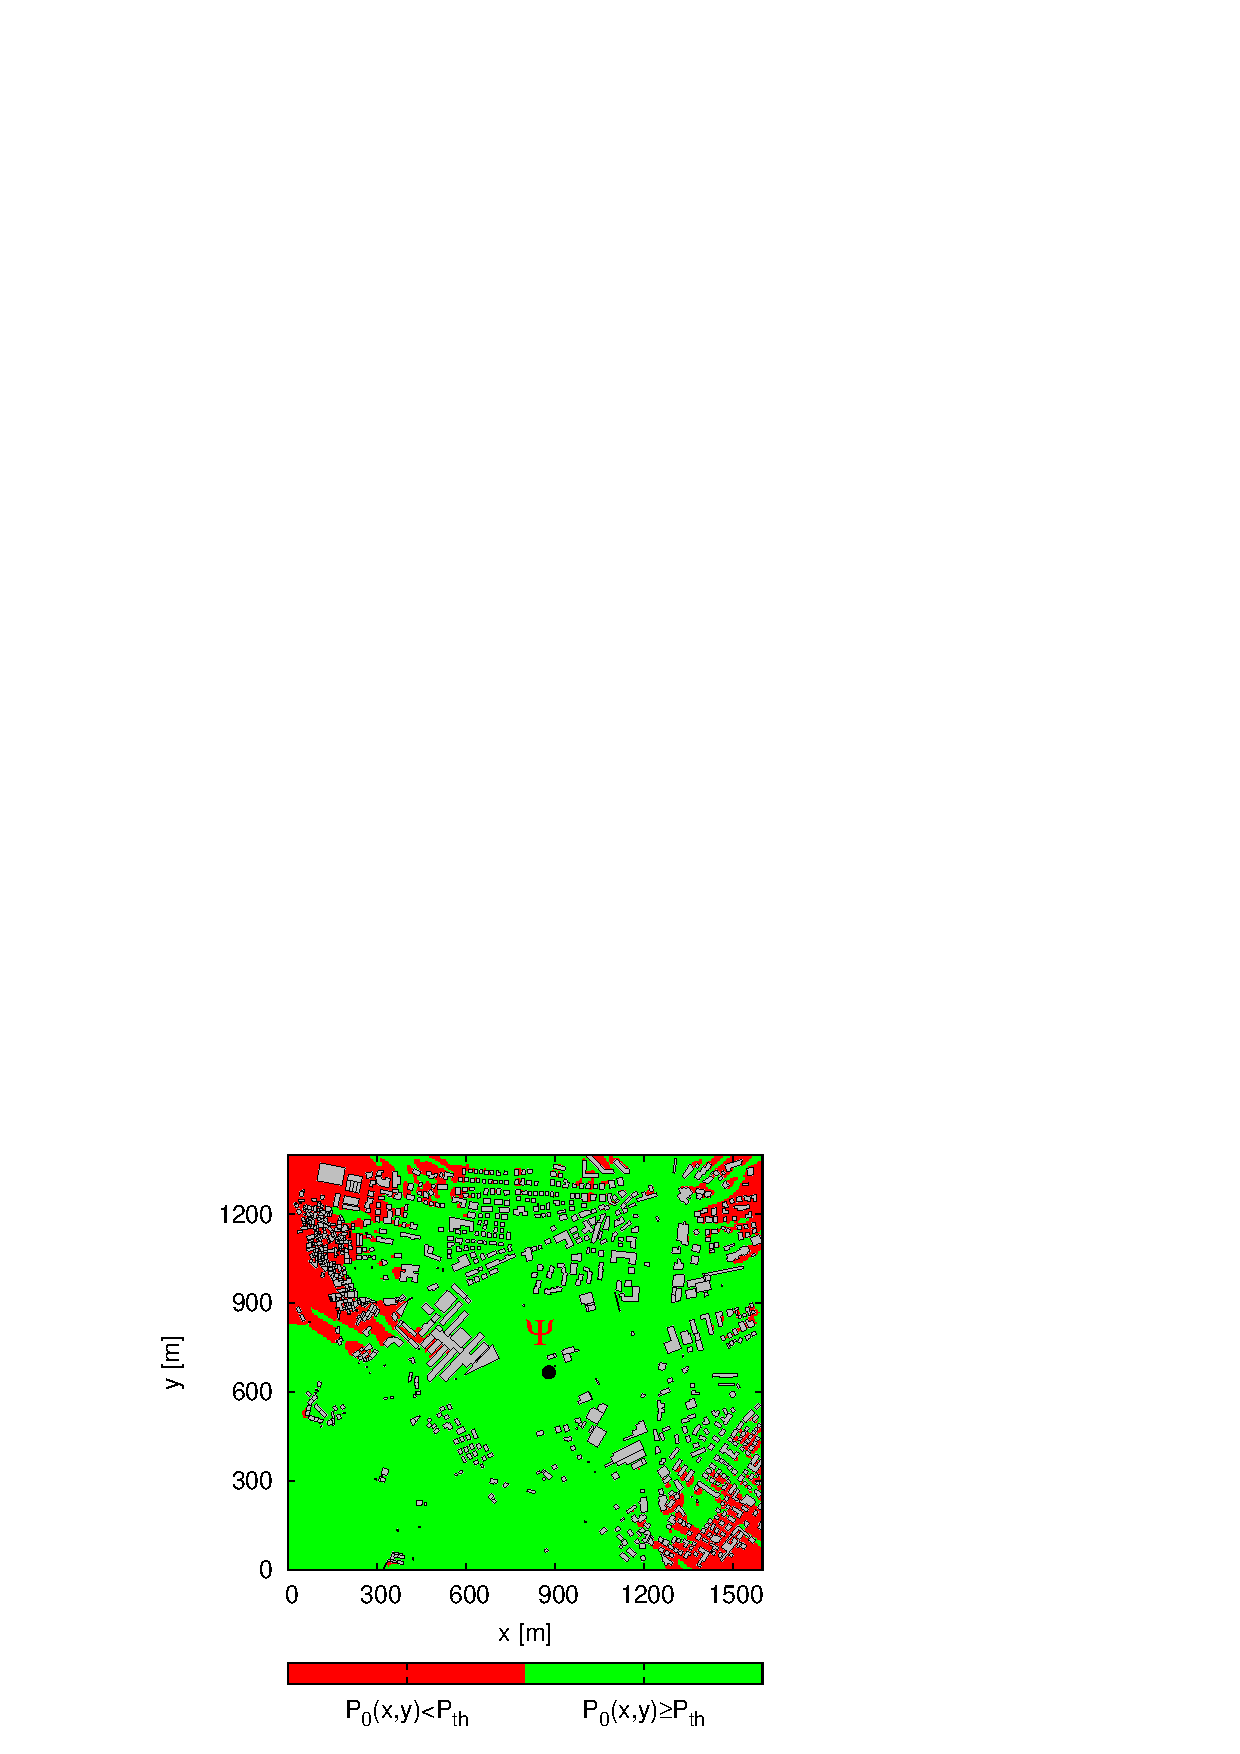
\includegraphics[scale=0.12]{./Figure/Planning.EM/Fig.Received.Power.Threshold.-65dBm.jpg}\tabularnewline
\emph{(a)}&
\emph{(b)}\tabularnewline
\end{tabular}\end{center}
\caption{\footnotesize \emph{(a)} Irradiated Power in Scenario \emph{- (b)} Thresholded
power at $-65[dB]$ in scenario }
\end{figure}
\subsection{Region of Interest}
Having chosen and modeled the scenario, the Regions of Interest,
or {}``RoIs'', needs to be found. 
\begin{figure}[H]
\begin{center}
\begin{tabular}{ccc}
\begin{sideways}RoI1\end{sideways}&
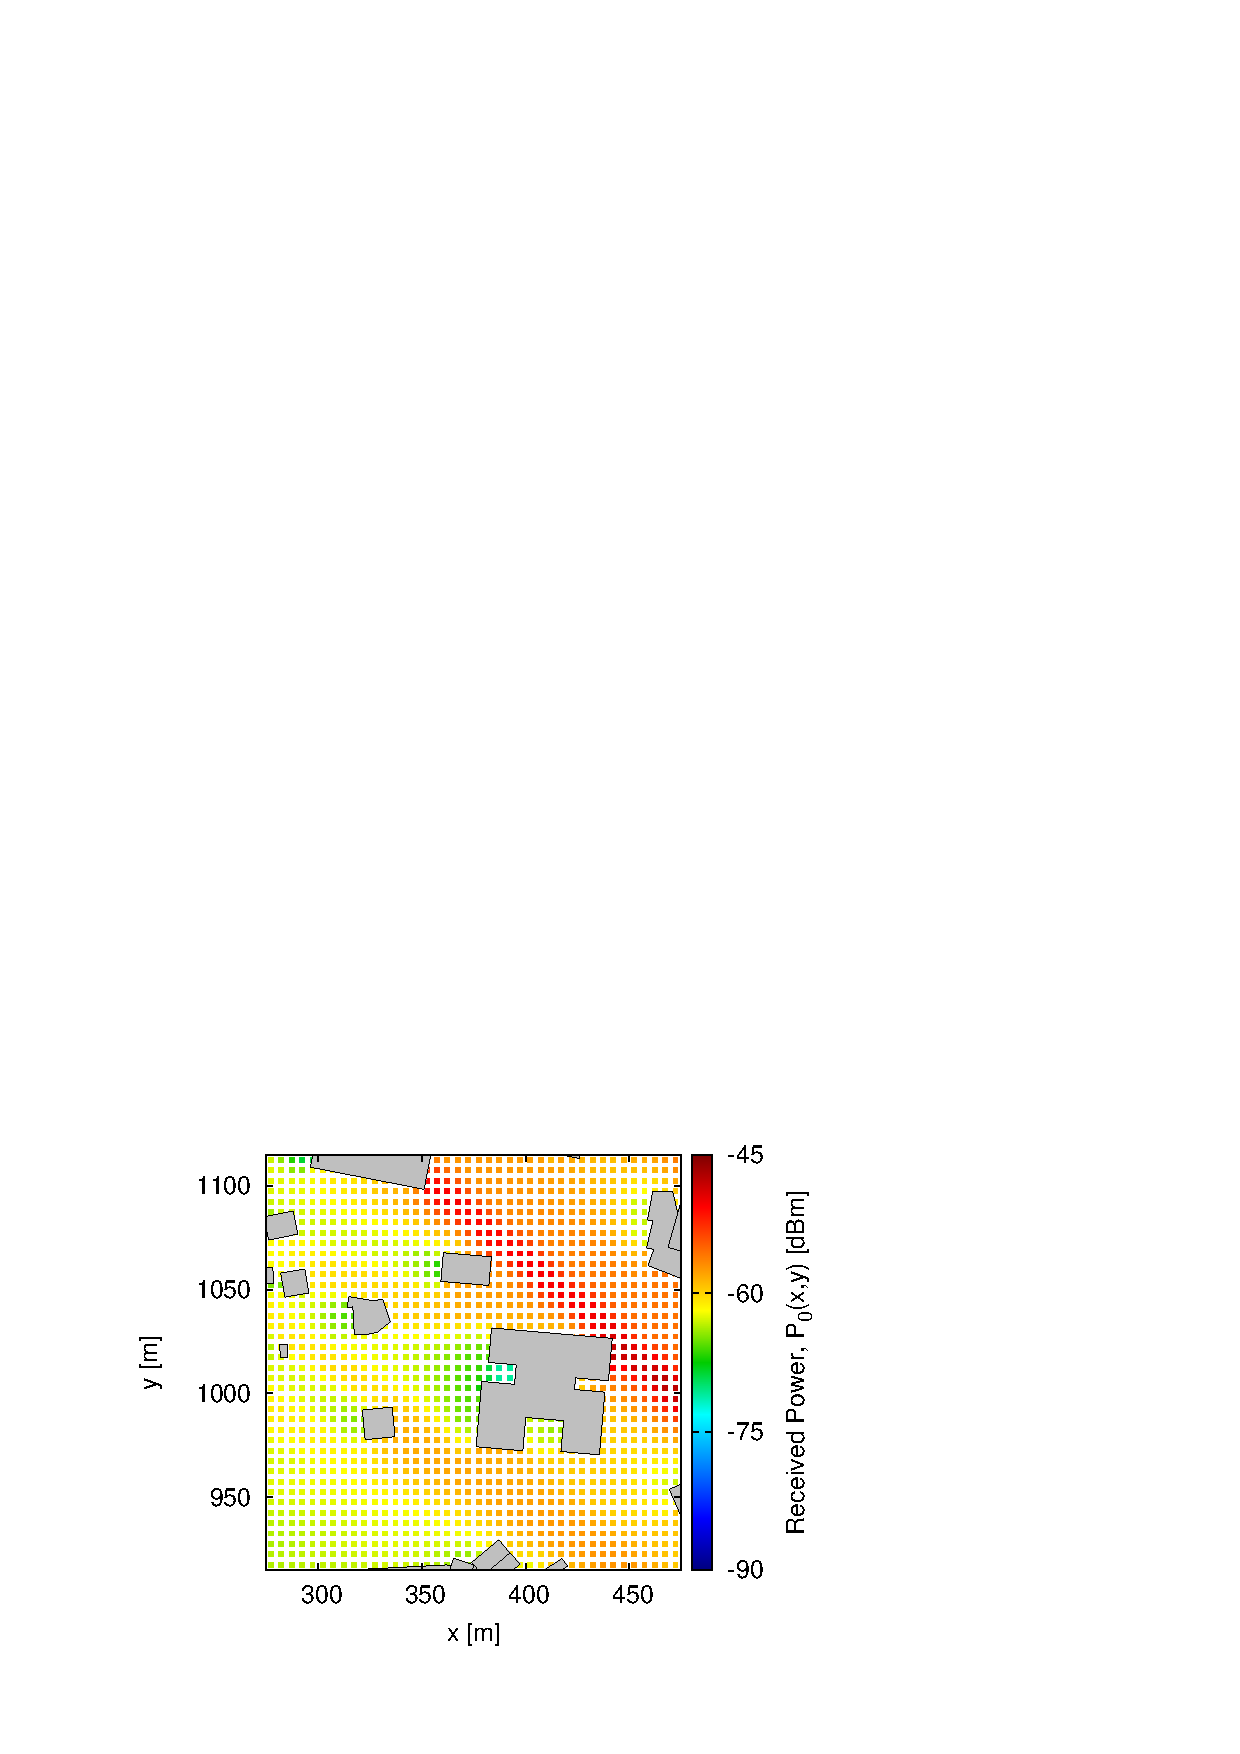
\includegraphics[scale=0.1]{./Figure/Planning.EM/RoI1/1/Fig.Received.Power.ZOOM.H-QoS-01.Reference.jpg}&\includegraphics[scale=0.1]{./Figure/Planning.EM/RoI1/1/Fig.Received.Power.ZOOM.RoI.Reference.Threshold.-65dBm.jpg}\tabularnewline
\begin{sideways}RoI2\end{sideways}&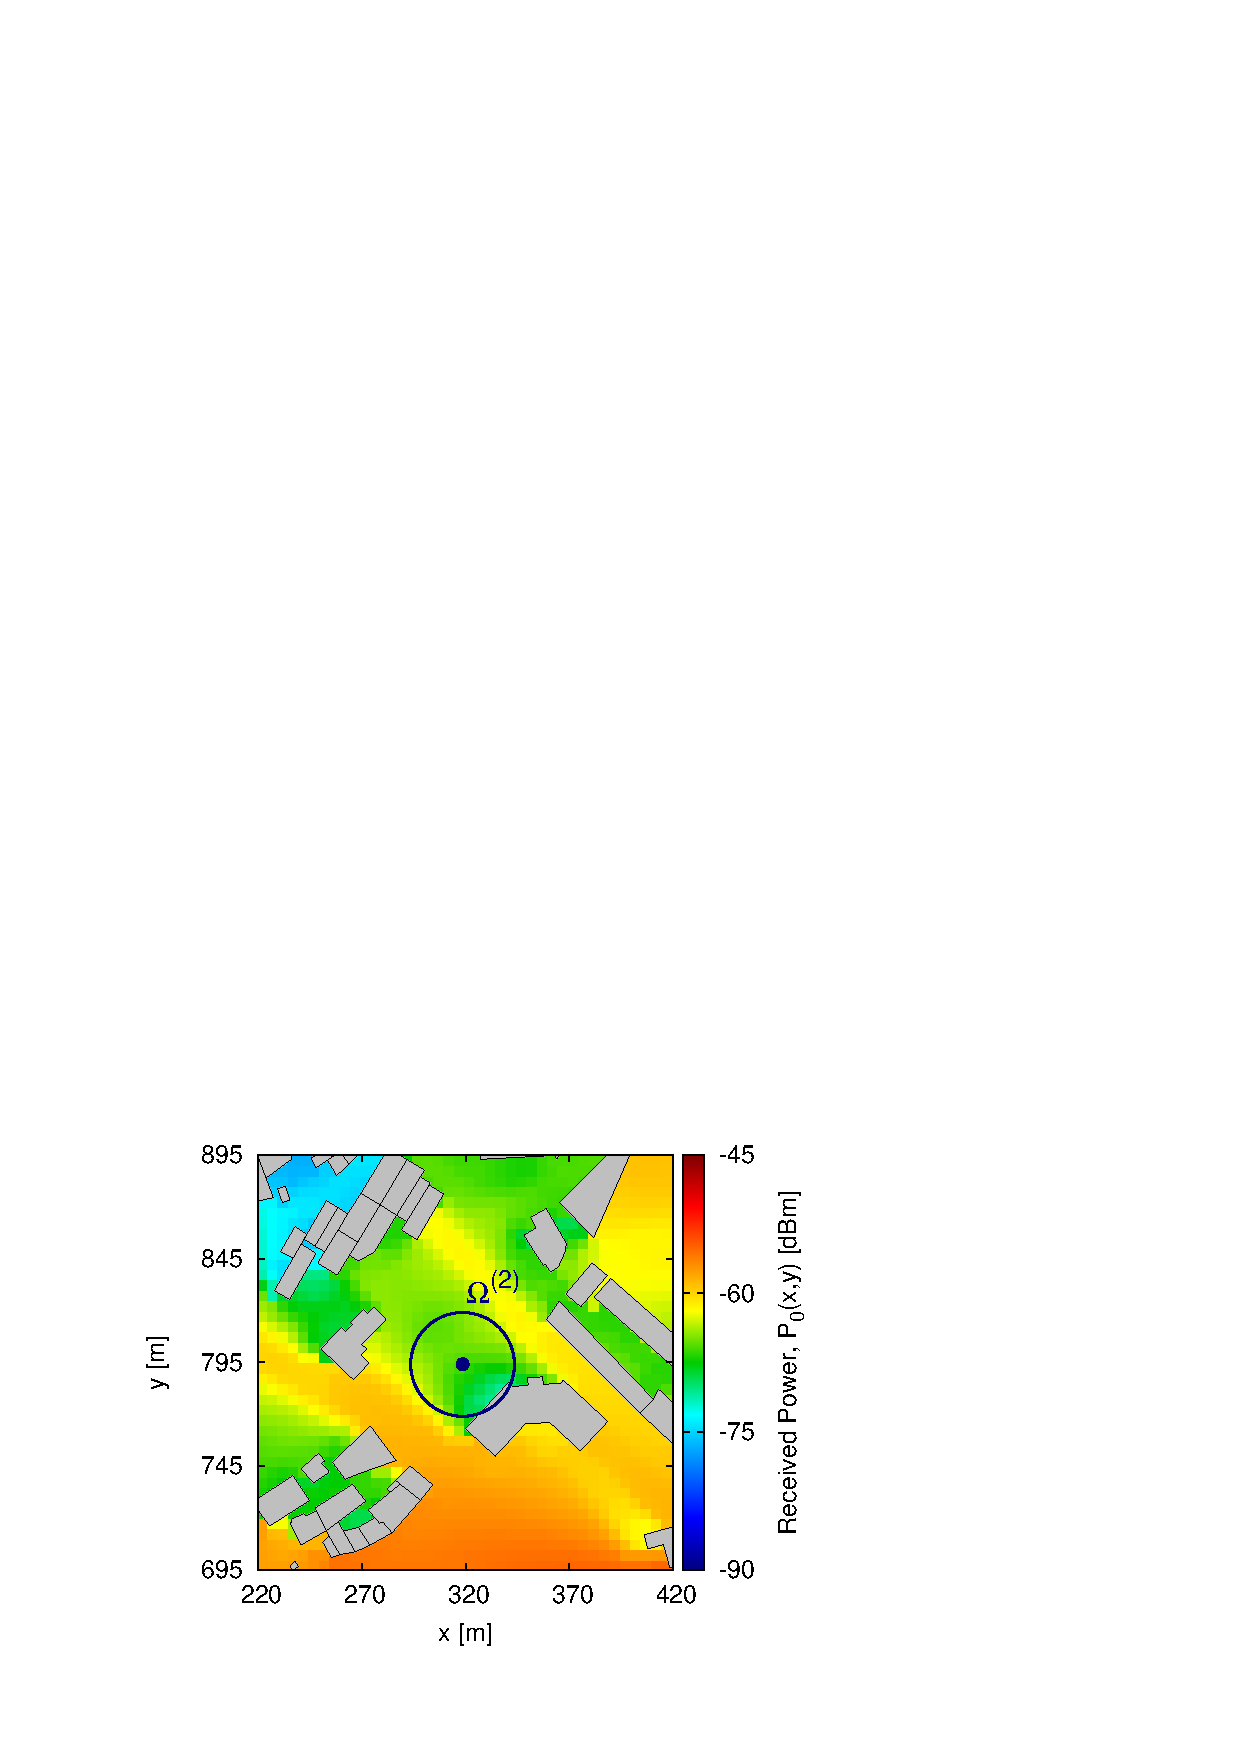
\includegraphics[scale=0.1]{./Figure/Planning.EM/RoI2/2/Fig.Received.Power.ZOOM.H-QoS-02.Reference.jpg}&\includegraphics[scale=0.1]{./Figure/Planning.EM/RoI2/2/Fig.Received.Power.ZOOM.RoI.Reference.Threshold.-65dBm.jpg}\tabularnewline
\begin{sideways}RoI3\end{sideways}&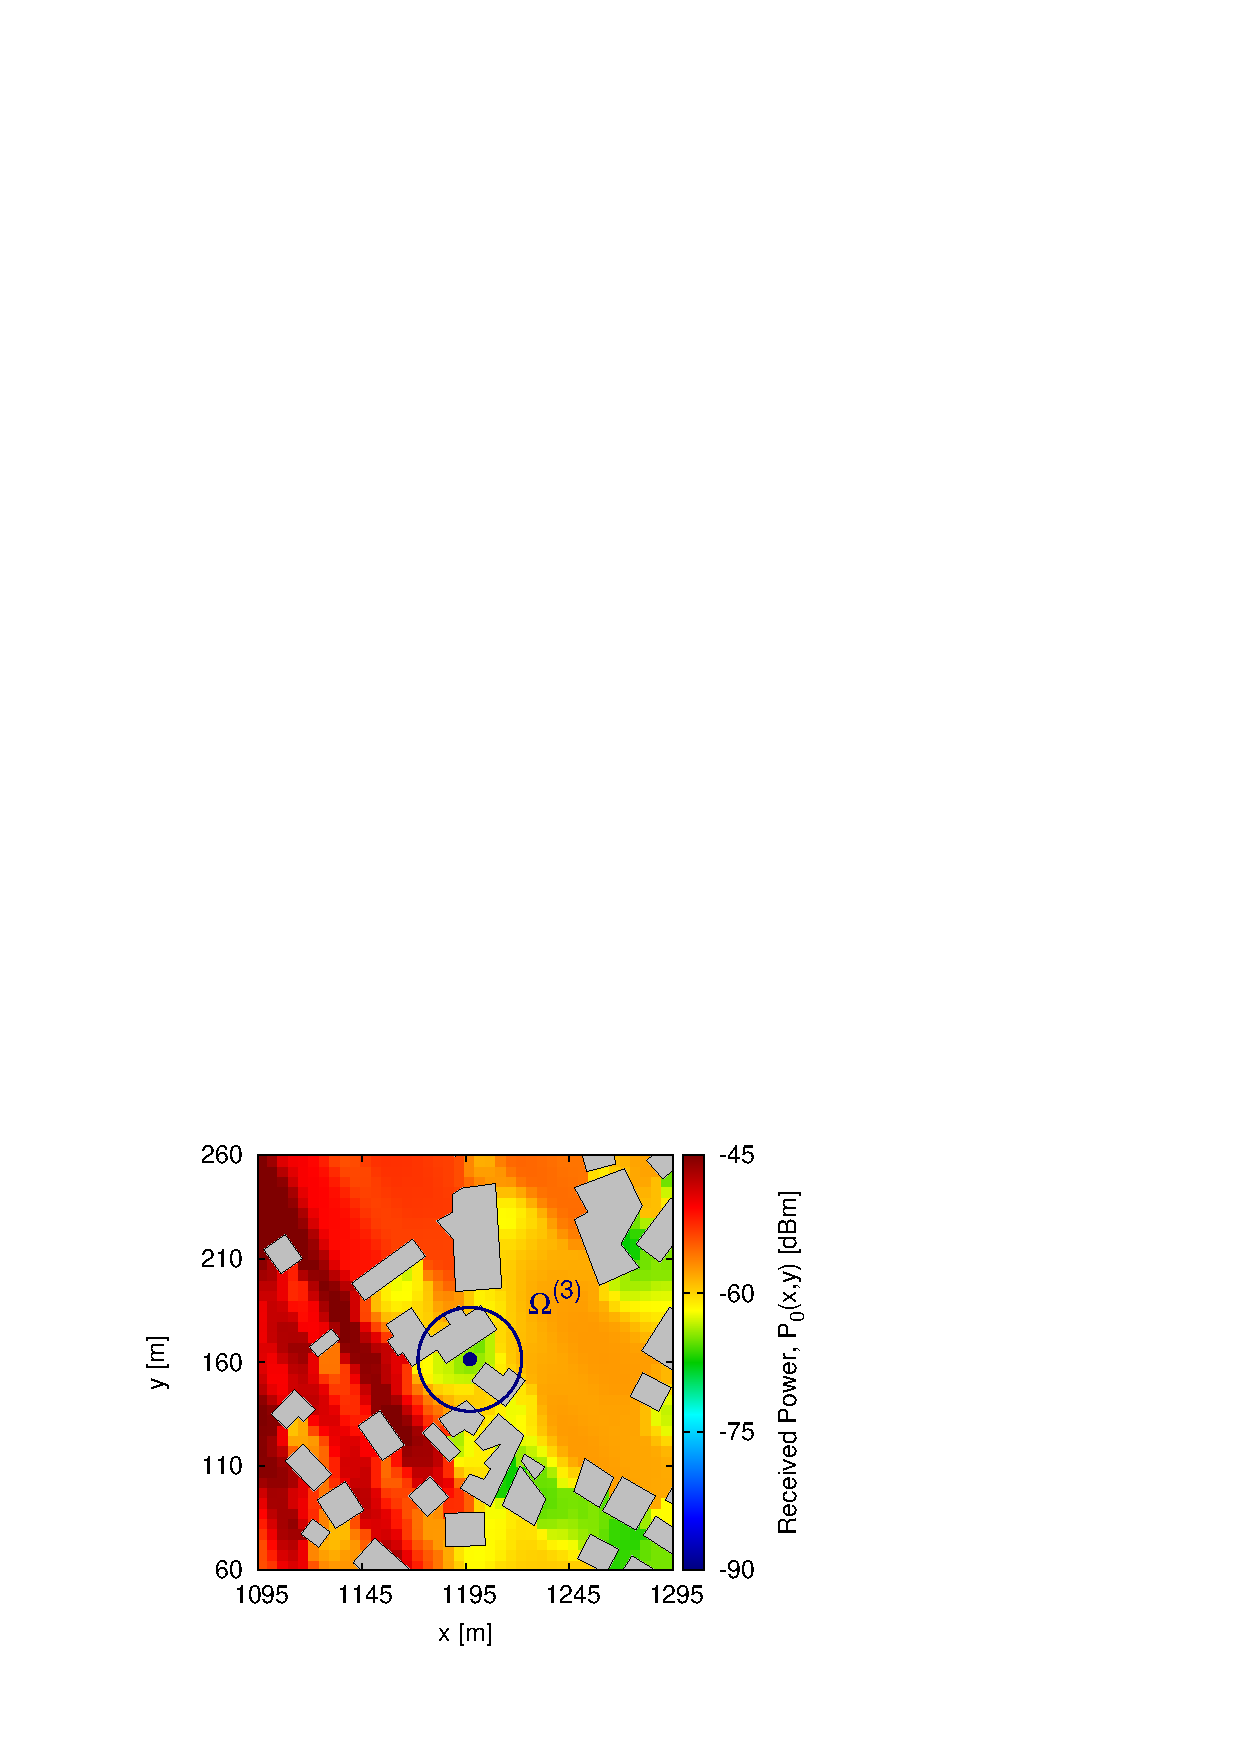
\includegraphics[scale=0.1]{./Figure/Planning.EM/RoI3/3/Fig.Received.Power.ZOOM.H-QoS-03.Reference.jpg}&\includegraphics[scale=0.1]{./Figure/Planning.EM/RoI3/3/Fig.Received.Power.ZOOM.RoI.Reference.Threshold.-65dBm.jpg}\tabularnewline
&\emph{(a)}&\emph{(b)}\tabularnewline
\end{tabular}\end{center}
\caption{\footnotesize \emph{(a)} Nominal Power for selected Region of Interest - \emph{(b)}
Thresholded power at $-65[dB]$ for selected Region of Interest}
\end{figure}


The following weak spots has been found, meaning that these spots
perform badly under -65{[}dBm{]}, which is the thresholded value used
in this discourse to determine if the BTS is working as supposed to.
Is crucial to maintain the signal above the threshold, otherwise the
BTS, and thus the ISP that owns the BTS, is incapable to provide a
minimum quality for the service, meaning that the user is going to
be affected. For example, the streaming video that the user is watching
will lag quite a bit if the received power in that zone is below -65{[}dBm{]}.
On the other hand, choosing spots with received power way above the
threshold is a waste of resources, since it's not needed to analyze,
model and test a EMS to improve said spot.


\subsection{Smart Skins Choice}

After defining the weak spots, or \char`\"{}Region of Interest\char`\"{},
the following step is to determine which wall is best suited to having
a EMS applied to it. Two criterias are mainly used for this step:
the proximity from the RoI, which the maximum value is ca. 70 meters,
and the Incident Power on said wall, which should be at least above
80 dB mu V/m, even though it's best to have it over 90 to ensure a
good amount of power reflected. 

Afterwards, when every RoI is deeply examined, all of the RoI characteristics
are going to be listed, showing the meaning behind the selection. 

%
\begin{figure}[H]
\begin{center}\begin{tabular}{cc}
\includegraphics[%
  scale=0.1]{./Figure/Planning.EM/RoI1/1/Fig.Scenario.ZOOM.H-QoS-01.Smart.Skins.jpg}&
\includegraphics[%
  scale=0.1]{./Figure/Planning.EM/RoI2/2/Fig.Scenario.ZOOM.H-QoS-02.Smart.Skins.jpg}\tabularnewline
(a)&
(b)\tabularnewline
\multicolumn{2}{c}{\includegraphics[%
  scale=0.1]{./Figure/Planning.EM/RoI3/3/Fig.Scenario.ZOOM.H-QoS-03.Smart.Skins.jpg}}\tabularnewline
\multicolumn{2}{c}{(c)}\tabularnewline
\end{tabular}\end{center}
\caption{\footnotesize \emph{(a)} Smart Skin Choice for Region Of Interest 1 \emph{- (b)}
Smart Skin Choice for Region Of Interest 2 \emph{- (c)} Smart Skin
Choice for Region Of Interest 3}
\end{figure}


%
\begin{figure}[H]
\begin{center}\begin{tabular}{c}
\includegraphics[scale=0.1]{./Figure/Planning.EM/Fig.Scenario.BTS.Rays.jpg}\tabularnewline
\emph{(a)}\tabularnewline
\end{tabular}\end{center}


\caption{\footnotesize \emph{(a)} Cumulative Smart Skin Choices}
\end{figure}



\subsection{Enhancement Region of Interest 1}

After defining all the characteristichs of the RoI, the next step
is to model the EMS, using the incident angles and the reflected angles.
The layout and the directivity of each EMS is shown, providing a view
of the direction which the EMS is intended to work. 


\subsubsection{Smart Skin Sizing and Layout}

%
\begin{table}[H]
\begin{center}\resizebox{\textwidth}{!}{\begin{tabular}{|c|c|c|c|}
\hline 
\#&
$\Gamma_{1}^{(1)}$&
$\Gamma_{2}^{(1)}$&
$\Gamma_{3}^{(1)}$\tabularnewline
\hline
Shape&
Square&
Square&
Square\tabularnewline
\hline
\emph{EMS} Side&
$d=2[m]$&
$d=2[m]$&
$d=2[m]$\tabularnewline
\hline
Number elements along $x$&
$N_{x}=50$&
$N_{x}=50$&
$N_{x}=50$\tabularnewline
\hline
Number elements along $y$&
$N_{y}=50$&
$N_{y}=50$&
$N_{y}=50$\tabularnewline
\hline
Distance from \emph{BTS}&
$D_{\Psi}=639.23[m]$&
$D_{\Psi}=658.91[m]$&
$D_{\Psi}=627.85[m]$\tabularnewline
\hline
Distance from RoI1&
$D_{\Omega}=40.26[m]$&
$D_{\Omega}=39[m]$&
$D_{\Omega}=47.04[m]$\tabularnewline
\hline
Incident angle&
$(\theta_{i},\phi_{i})=(57.33,1.60)[deg]$&
$(\theta_{i},\phi_{i})=(16.72,4.54)[deg]$&
$(\theta_{i},\phi_{i})=(34.02,177.55)[deg]$\tabularnewline
\hline
Reflection angle&
$(\theta_{r},\phi_{r})=(20.23,-104.13)[deg]$&
$(\theta_{r},\phi_{r})=(30.67,-42.74)[deg]$&
$(\theta_{r},\phi_{r})=(49.47,-22.18)[deg]$\tabularnewline
\hline
\emph{EMS} Location&
$(x_{\Gamma},y_{\Gamma},z_{\Gamma})=(334,979,15)[m]$&
$(x_{\Gamma},y_{\Gamma},z_{\Gamma})=(330,1030,15)[m]$&
$(x_{\Gamma},y_{\Gamma},z_{\Gamma})=(369,1051,15)[m]$\tabularnewline
\hline
Incident field strength&
$E_{rms}=89.47[dB\mu V/m]$&
$E_{rms}=86.26[dB\mu V/m]$&
$E_{rms}=96.49[dB\mu V/m]$\tabularnewline
\hline
Reflected power&
$P_{\Gamma}=-20.27[dBm]$&
$P_{\Gamma}=-19.42[dBm]$&
$P_{\Gamma}=-13.76[dBm]$\tabularnewline
\hline
\end{tabular}}\end{center}


\caption{\footnotesize Region of Interest 1 data}
\end{table}


%
\begin{figure}[H]
\begin{center}\begin{tabular}{ccc}
\begin{sideways}
\textcolor{white}{xxxxxx}$\Gamma_{1}^{(1)}$%
\end{sideways}&
\includegraphics[%
  scale=0.1]{./Figure/Planning.EM/RoI1/1_1/Fig.SQUARE.PATCH-50x50.EMS-Layout1.1.jpg}&
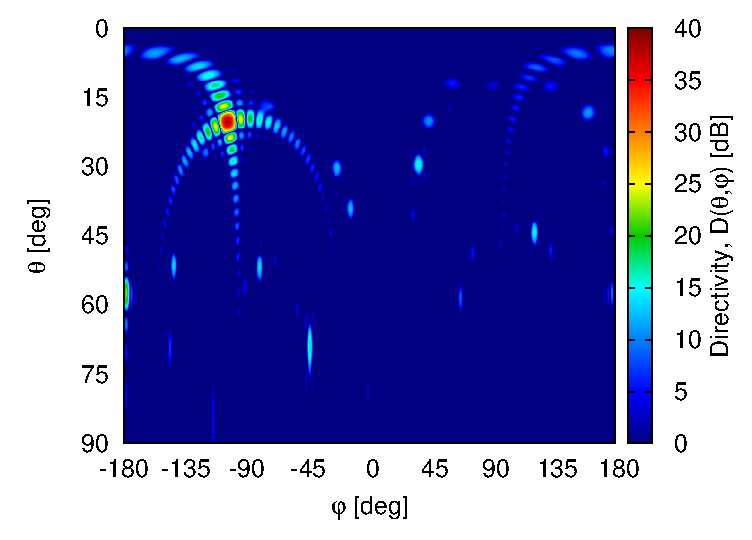
\includegraphics[%
  scale=0.1]{./Figure/Planning.EM/RoI1/1_1/Fig.Directivity.EMS1.1.jpg}\tabularnewline
\begin{sideways}
\textcolor{white}{xxxxxx}$\Gamma_{2}^{(1)}$%
\end{sideways}&
\includegraphics[%
  scale=0.1]{./Figure/Planning.EM/RoI1/1_2/Fig.SQUARE.PATCH-50x50.EMS-Layout1.2.jpg}&
\includegraphics[%
  scale=0.1]{./Figure/Planning.EM/RoI1/1_2/Fig.Directivity.EMS1.2.jpg}\tabularnewline
\begin{sideways}
\textcolor{white}{xxxxxx}$\Gamma_{3}^{(1)}$%
\end{sideways}&
\includegraphics[%
  scale=0.1]{./Figure/Planning.EM/RoI1/1_3/Fig.SQUARE.PATCH-50x50.EMS-Layout1.3.jpg}&
\includegraphics[%
  scale=0.1]{./Figure/Planning.EM/RoI1/1_3/Fig.Directivity.EMS1.3.jpg}\tabularnewline
&
\emph{(a)}&
\begin{sideways}
\emph{(b)}%
\end{sideways}\tabularnewline
\end{tabular}\end{center}

\vspace{-10pt}
\caption{\footnotesize \emph{(a)} Layout - \emph{(b)} Directivity}
\end{figure}



\subsubsection{Smart Skin Performance}

%
\begin{figure}[H]
\begin{center}\resizebox{\textwidth}{!}{\begin{tabular}{cccc}
\begin{sideways}
\textcolor{white}{xxxxxx}Nominal%
\end{sideways}&
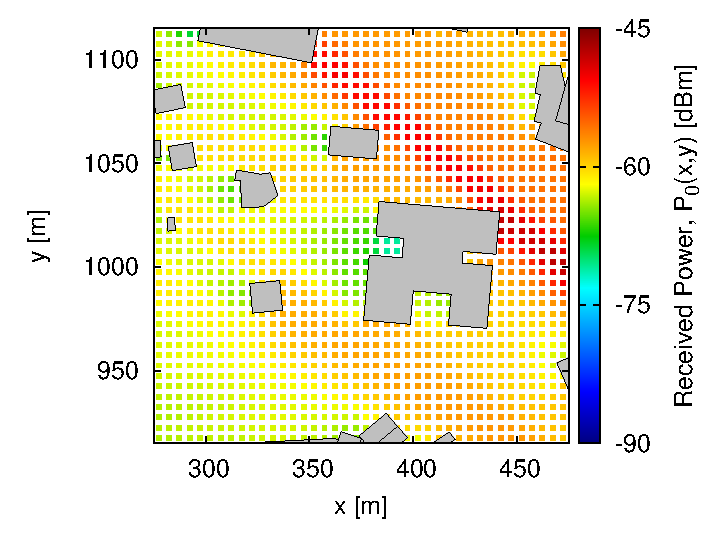
\includegraphics[%
  scale=0.55]{./Figure/Planning.EM/RoI1/1/Fig.Received.Power.ZOOM.H-QoS-01.Reference.jpg}&
\includegraphics[%
  scale=0.53]{./Figure/Planning.EM/RoI1/1/Fig.Received.Power.ZOOM.RoI.Reference.Threshold.-65dBm.jpg}&
\tabularnewline
\begin{sideways}
\textcolor{white}{xxxxxx}$\Gamma_{1}^{(1)}$%
\end{sideways}&
\includegraphics[%
  scale=0.55]{./Figure/Planning.EM/RoI1/1_1/Fig.Received.Power.ZOOM.RoI.Planning.EM.-65dBm.jpg}&
\includegraphics[%
  scale=0.53]{./Figure/Planning.EM/RoI1/1_1/Fig.Received.Power.ZOOM.RoI.Planning.EM.Threshold.-65dBm.jpg}&
\includegraphics[%
  scale=0.53]{./Figure/Planning.EM/RoI1/1_1/Fig.Difference.Received.Power.ZOOM.RoI.Threshold.-65dBm.Planning.EM.vs.Reference.jpg}\tabularnewline
\begin{sideways}
\textcolor{white}{xxxxxx}$\Gamma_{2}^{(1)}$%
\end{sideways}&
\includegraphics[%
  scale=0.55]{./Figure/Planning.EM/RoI1/1_2/Fig.Received.Power.ZOOM.RoI.Planning.EM.-65dBm.jpg}&
\includegraphics[%
  scale=0.53]{./Figure/Planning.EM/RoI1/1_2/Fig.Received.Power.ZOOM.RoI.Planning.EM.Threshold.-65dBm.jpg}&
\includegraphics[%
  scale=0.53]{./Figure/Planning.EM/RoI1/1_2/Fig.Difference.Received.Power.ZOOM.RoI.Threshold.-65dBm.Planning.EM.vs.Reference.jpg}\tabularnewline
\begin{sideways}
\textcolor{white}{xxxxxx}$\Gamma_{3}^{(1)}$%
\end{sideways}&
\includegraphics[%
  scale=0.55]{./Figure/Planning.EM/RoI1/1_3/Fig.Received.Power.ZOOM.RoI.Planning.EM.-65dBm.jpg}&
\includegraphics[%
  scale=0.53]{./Figure/Planning.EM/RoI1/1_3/Fig.Received.Power.ZOOM.RoI.Planning.EM.Threshold.-65dBm.jpg}&
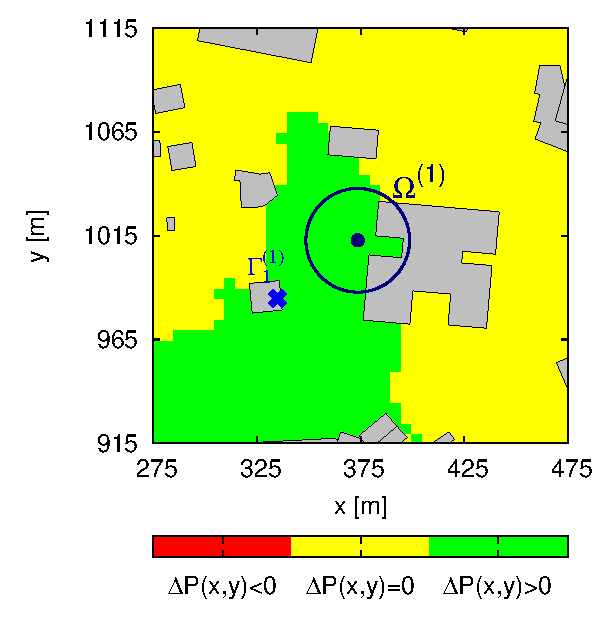
\includegraphics[%
  scale=0.53]{./Figure/Planning.EM/RoI1/1_3/Fig.Difference.Received.Power.ZOOM.RoI.Threshold.-65dBm.Planning.EM.vs.Reference.jpg}\tabularnewline
&
(a)&
(b)&
(c)\tabularnewline
\end{tabular}}\end{center}


\caption{\footnotesize (a) Nominal BTS Power Performance vs Smart Skin Performance in Region
of Interest 1 - \emph{(b)} (a) Nominal BTS Thresholded Power Performance
vs Thresholded Smart Skin Performance in Region of Interest 1 - \emph{(c)}
Difference between received and reflected power thresholded at $-65[dBm]$}
\end{figure}


Having applied the modelled EMSs in each inteded spot, it's clear
that an improvement has been made, especially with $\Gamma_{3}^{(1)}$,
which is going to be chosed as best performing EMS.

%
\subsubsection{Best Skin and Overall Implementation}
A scenario with all of the EMSs is show, with the thresholded map
and the difference between the Reference Scenario and the Improved
Scenario.
%
\begin{figure}[H]
\begin{center}\begin{tabular}{ccc}
Best Skin &
Threshold&
Difference\tabularnewline
\includegraphics[%
  scale=0.1]{./Figure/Planning.EM/RoI1/1_3/Fig.Received.Power.ZOOM.RoI.Planning.EM.Threshold.-65dBm.jpg}&
\includegraphics[%
  scale=0.1]{./Figure/Planning.EM/RoI1/1/Fig.Received.Power.ZOOM.RoI.Planning.EM.Threshold.-65dBm.jpg}&
\includegraphics[%
  scale=0.1]{./Figure/Planning.EM/RoI1/1/Fig.Difference.Received.Power.ZOOM.RoI.Threshold.-65dBm.Planning.EM.vs.Reference.jpg}\tabularnewline
\emph{(a)}&
\emph{(b)}&
\emph{(c)}\tabularnewline
\multicolumn{3}{c}{CDF}\tabularnewline
\multicolumn{3}{c}{\includegraphics[%
  scale=0.1]{./Figure/Planning.EM/RoI1/1/Fig.Cumulative.Density.Function.RoI.Threshold.-65dBm.jpg}}\tabularnewline
\multicolumn{3}{c}{\emph{(d)}}\tabularnewline
\end{tabular}\end{center}


\caption{\footnotesize \emph{(a)} - Best Skin for examined Scenario \emph{(b)} Environment with Smart Skins \emph{- (c)} Difference between
referenced and smart skin implemented Region of Interest - \emph{(d)}
Cumulative Density Function {[}-65dBm{]}}
\end{figure}


The difference between Referenced and EMSs implemented RoI is very
useful, not only to see the improvement in the RoI but even in other
places surrounding the EMSs. 

A graph for the CDF, Cumulative Density Function, is shown, stating
the probability that a point inside the RoI is going the threshold
value. For example, with all the EMSs applied, the CDF is ca. 17\%
in the RoI, much better than the referenced scenario, which was ca.
33\%. 


\subsection{Enhancement Region of Interest 2}
\subsubsection{Smart Skin Sizing and Layout}
\begin{table}[H]
\begin{center}\resizebox{\textwidth}{!}{\begin{tabular}{|c|c|c|c|c|}
\hline 
\#&
$\Gamma_{1}^{(2)}$&
$\Gamma_{2}^{(2)}$&
$\Gamma_{3}^{(2)}$&
$\Gamma_{4}^{(2)}$\tabularnewline
\hline
Shape&
Square&
Square&
Square&
Square\tabularnewline
\hline
\emph{EMS} Side&
$d=2[m]$&
$d=2[m]$&
$d=2[m]$&
$d=2[m]$\tabularnewline
\hline
Number elements along $x$&
$N_{x}=50$&
$N_{x}=50$&
$N_{x}=50$&
$N_{x}=50$\tabularnewline
\hline
Number elements along $y$&
$N_{y}=50$&
$N_{y}=50$&
$N_{y}=50$&
$N_{y}=50$\tabularnewline
\hline
Distance from \emph{BTS}&
$D_{\Psi}=610.74[m]$&
$D_{\Psi}=621.01[m]$&
$D_{\Psi}=606.90[m]$&
$D_{\Psi}=586.72[m]$\tabularnewline
\hline
Distance from RoI2&
$D_{\Omega}=73.02[m]$&
$D_{\Omega}=48.02[m]$&
$D_{\Omega}=57.88[m]$&
$D_{\Omega}=60.65[m]$\tabularnewline
\hline
Incident angle&
$(\theta_{i},\phi_{i})=(11.19,7.27)[deg]$&
$(\theta_{i},\phi_{i})=(28.25,2.92)[deg]$&
$(\theta_{i},\phi_{i})=(45.51,178.01)[deg]$&
$(\theta_{i},\phi_{i})=(59.52,178.30)[deg]$\tabularnewline
\hline
Reflection angle&
$(\theta_{r},\phi_{r})=(47.07,-165.37)[deg]$&
$(\theta_{r},\phi_{r})=(28.50,-36.10)[deg]$&
$(\theta_{r},\phi_{r})=(15.57,-60.33)[deg]$&
$(\theta_{r},\phi_{r})=(20.65,-39.14)[deg]$\tabularnewline
\hline
\emph{EMS} Location&
$(x_{\Gamma},y_{\Gamma},z_{\Gamma})=(297,864,15)[m]$&
$(x_{\Gamma},y_{\Gamma},z_{\Gamma})=(275,808,15)[m]$&
$(x_{\Gamma},y_{\Gamma},z_{\Gamma})=(279,754,15)[m]$&
$(x_{\Gamma},y_{\Gamma},z_{\Gamma})=(301,739)[m]$\tabularnewline
\hline
Incident field strength&
$E_{rms}=94.3[dB\mu V/m]$&
$E_{rms}=89.76[dB\mu V/m]$&
$E_{rms}=89.95[dB\mu V/m]$&
$E_{rms}=81.31[dB\mu V/m]$\tabularnewline
\hline
Reflected power&
$P_{\Gamma}=-15.50[dBm]$&
$P_{\Gamma}=-17.80[dBm]$&
$P_{\Gamma}=-20.08[dBm]$&
$P_{\Gamma}=-21.30[dBm]$\tabularnewline
\hline
\end{tabular}}\end{center}

\caption{\footnotesize Region of Interest 2 data}
\end{table}

\begin{figure}[H]
\begin{center}\begin{tabular}{ccc}
\begin{sideways}
\textcolor{white}{xxxxxx}$\Gamma_{1}^{(2)}$\end{sideways}&
\includegraphics[%
  scale=0.1]{./Figure/Planning.EM/RoI2/2_1/Fig.SQUARE.PATCH-50x50.EMS-Layout2.1.jpg}&
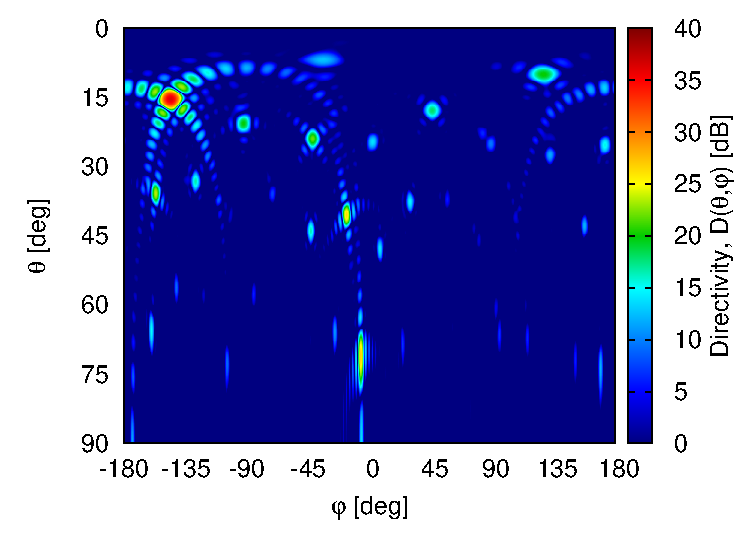
\includegraphics[%
  scale=0.1]{./Figure/Planning.EM/RoI2/2_1/Fig.Directivity.EMS2.1.jpg}\tabularnewline
\begin{sideways}
\textcolor{white}{xxxxxx}$\Gamma_{2}^{(2)}$%
\end{sideways}&
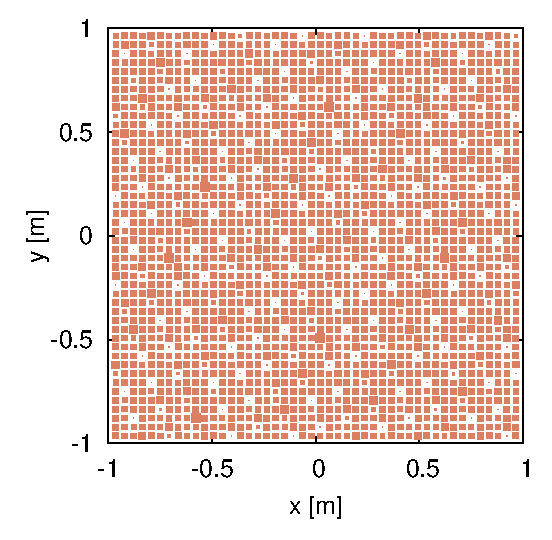
\includegraphics[%
  scale=0.1]{./Figure/Planning.EM/RoI2/2_2/Fig.SQUARE.PATCH-50x50.EMS-Layout2.2.jpg}&
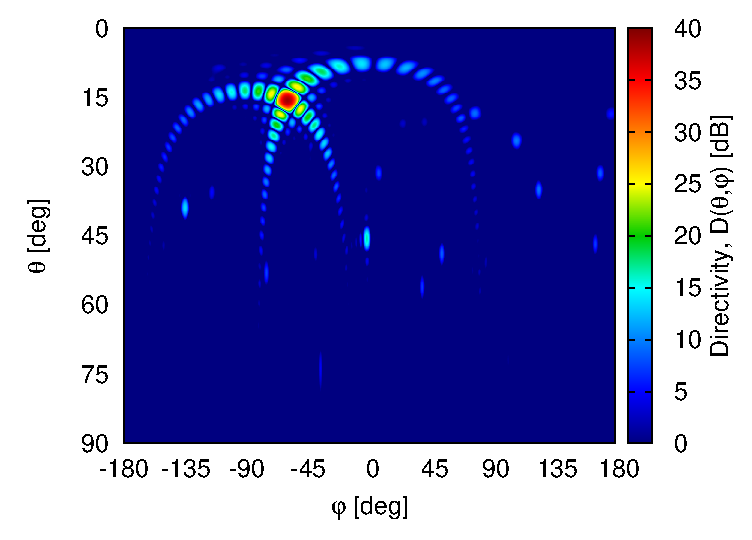
\includegraphics[%
  scale=0.1]{./Figure/Planning.EM/RoI2/2_2/Fig.Directivity.EMS2.2.jpg}\tabularnewline
\begin{sideways}
\textcolor{white}{xxxxxxx}$\Gamma_{3}^{(2)}$%
\end{sideways}&
\includegraphics[%
  scale=0.1]{./Figure/Planning.EM/RoI2/2_3/Fig.SQUARE.PATCH-50x50.EMS-Layout2.3.jpg}&
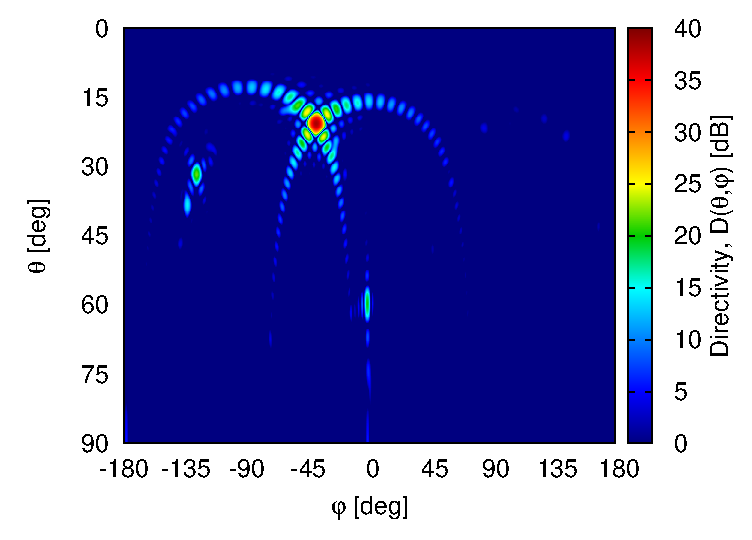
\includegraphics[%
  scale=0.1]{./Figure/Planning.EM/RoI2/2_3/Fig.Directivity.EMS2.3.jpg}\tabularnewline
\begin{sideways}
\textcolor{white}{xxxxxx}$\Gamma_{4}^{(2)}$%
\end{sideways}&
\includegraphics[%
  scale=0.1]{./Figure/Planning.EM/RoI2/2_4/Fig.SQUARE.PATCH-50x50.EMS-Layout2.4.jpg}&
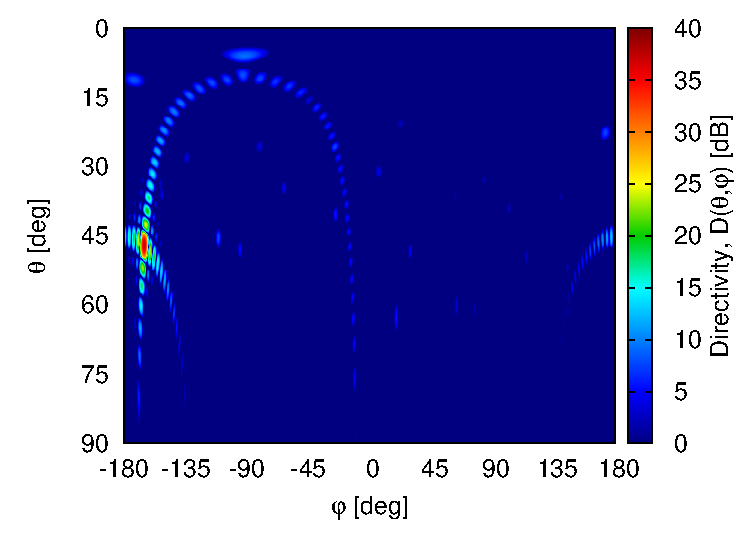
\includegraphics[%
  scale=0.1]{./Figure/Planning.EM/RoI2/2_4/Fig.Directivity.EMS2.4.jpg}\tabularnewline
&
\emph{(a)}&
\emph{(b)}\tabularnewline
\end{tabular}\end{center}


\caption{\emph{(a)} Layout - \emph{(b)} Directivity}
\end{figure}

\subsubsection{Smart Skins Performance}

\begin{figure}[H]
\begin{center}\begin{tabular}{cccc}
\begin{sideways}
\textcolor{white}{xxxxxxx}Nominal%
\end{sideways}&
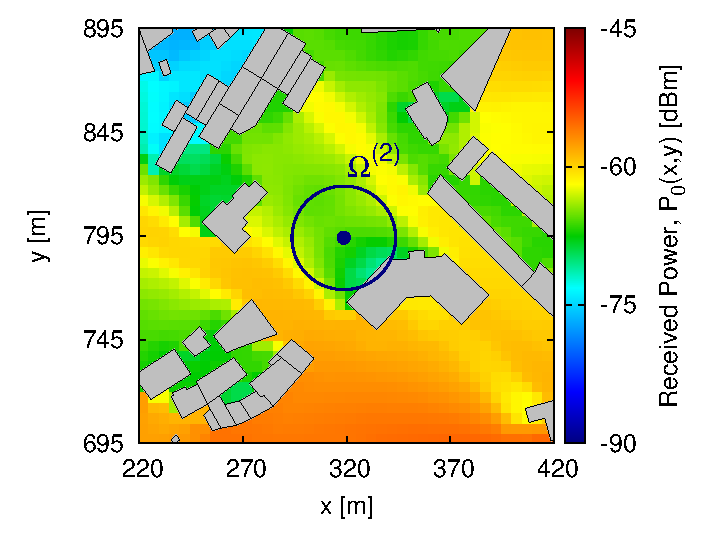
\includegraphics[%
  scale=0.08]{./Figure/Planning.EM/RoI2/2/Fig.Received.Power.ZOOM.H-QoS-02.Reference.jpg}&
\includegraphics[%
  scale=0.08]{./Figure/Planning.EM/RoI2/2_1/Fig.Received.Power.ZOOM.RoI.Planning.EM.Threshold.-65dBm.jpg}&
\tabularnewline
\begin{sideways}
\textcolor{white}{xxxxxxxxxxx}$\Gamma_{1}^{(2)}$%
\end{sideways}&
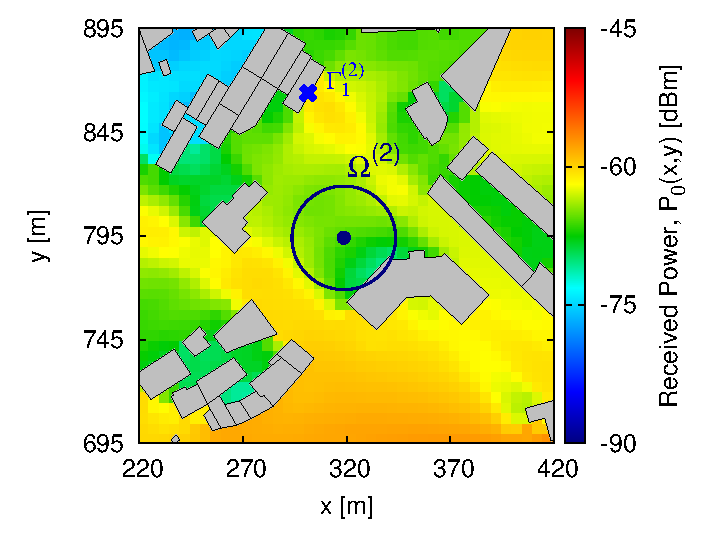
\includegraphics[%
  scale=0.08]{./Figure/Planning.EM/RoI2/2_1/Fig.Received.Power.ZOOM.H-QoS-02.Reference.jpg}&
\includegraphics[%
  scale=0.08]{./Figure/Planning.EM/RoI2/2_1/Fig.Received.Power.ZOOM.RoI.Planning.EM.Threshold.-65dBm.jpg}&
\includegraphics[%
  scale=0.08]{./Figure/Planning.EM/RoI2/2_1/Fig.Difference.Received.Power.ZOOM.RoI.Threshold.-65dBm.Planning.EM.vs.Reference.jpg}\tabularnewline
\begin{sideways}
\textcolor{white}{xxxxxxxxxx}$\Gamma_{2}^{(2)}$%
\end{sideways}&
\includegraphics[%
  scale=0.08]{./Figure/Planning.EM/RoI2/2_2/Fig.Received.Power.ZOOM.H-QoS-02.Reference.jpg}&
\includegraphics[%
  scale=0.08]{./Figure/Planning.EM/RoI2/2_2/Fig.Received.Power.ZOOM.RoI.Planning.EM.Threshold.-65dBm.jpg}&
\includegraphics[%
  scale=0.08]{./Figure/Planning.EM/RoI2/2_2/Fig.Difference.Received.Power.ZOOM.RoI.Threshold.-65dBm.Planning.EM.vs.Reference.jpg}\tabularnewline
  \begin{sideways}
\textcolor{white}{xxxxxxxxx}$\Gamma_{3}^{(2)}$%
\end{sideways}&
\includegraphics[%
  scale=0.08]{./Figure/Planning.EM/RoI2/2_3/Fig.Received.Power.ZOOM.H-QoS-02.Reference.jpg}&
\includegraphics[%
  scale=0.08]{./Figure/Planning.EM/RoI2/2_3/Fig.Received.Power.ZOOM.RoI.Planning.EM.Threshold.-65dBm.jpg}&
\includegraphics[%
  scale=0.08]{./Figure/Planning.EM/RoI2/2_3/Fig.Difference.Received.Power.ZOOM.RoI.Threshold.-65dBm.Planning.EM.vs.Reference.jpg}\tabularnewline
\begin{sideways}
\textcolor{white}{xxxxxxxxx}$\Gamma_{4}^{(2)}$%
\end{sideways}&
\includegraphics[%
  scale=0.08]{./Figure/Planning.EM/RoI2/2_4/Fig.Received.Power.ZOOM.H-QoS-02.Reference.jpg}&
\includegraphics[%
  scale=0.08]{./Figure/Planning.EM/RoI2/2_4/Fig.Received.Power.ZOOM.RoI.Planning.EM.Threshold.-65dBm.jpg}&
\includegraphics[%
  scale=0.08]{./Figure/Planning.EM/RoI2/2_4/Fig.Difference.Received.Power.ZOOM.RoI.Threshold.-65dBm.Planning.EM.vs.Reference.jpg}\tabularnewline
&
(a)&
(b)&
(c)\tabularnewline
\end{tabular}\end{center}

\vspace{-15pt}
\caption{\footnotesize (a) Nominal BTS Power Performance vs Smart Skin Performance in Region
of Interest 2 - \emph{(b)} (a) Nominal BTS Thresholded Power Performance
vs Thresholded Smart Skin Performance in Region of Interest 2 - \emph{(c)}
Difference between received and reflected power thresholded at $-65[dBm]$}
\end{figure}


\subsubsection{Best Skin and Overall Implementation}

%
\begin{figure}[H]
\begin{center}\begin{tabular}{ccc}
Best Skin&
Threshold&
Difference\tabularnewline
\includegraphics[%
  scale=0.1]{./Figure/Planning.EM/RoI2/2_1/Fig.Received.Power.ZOOM.RoI.Planning.EM.Threshold.-65dBm.jpg}&
\includegraphics[%
  scale=0.1]{./Figure/Planning.EM/RoI2/2/Fig.Received.Power.ZOOM.RoI.Planning.EM.Threshold.-65dBm.jpg}&
\includegraphics[%
  scale=0.1]{./Figure/Planning.EM/RoI2/2/Fig.Difference.Received.Power.ZOOM.RoI.Threshold.-65dBm.Planning.EM.vs.Reference.jpg}\tabularnewline
\emph{(a)}&
\emph{(b)}&
\emph{(c)}\tabularnewline
\multicolumn{3}{c}{CDF}\tabularnewline
\multicolumn{3}{c}{\includegraphics[%
  scale=0.1]{./Figure/Planning.EM/RoI2/2/Fig.Cumulative.Density.Function.RoI.Threshold.-65dBm.jpg}}\tabularnewline
\multicolumn{3}{c}{\emph{(d)}}\tabularnewline
\end{tabular}\end{center}


\caption{\footnotesize \emph{(a)} - Best Skin for examined Scenario \emph{(b)} Environment with Smart Skins \emph{- (c)} Difference between
referenced and smart skin implemented Region of Interest - \emph{(d)}
Cumulative Density Function {[}-65dBm{]}}
\end{figure}



\subsection{Enhancement Region of Interest 3}


\subsubsection{Smart Skin Sizing and Layout}

%
\begin{table}[H]
\begin{center}\resizebox{\textwidth}{!}{\begin{tabular}{|c|c|c|}
\hline 
\#&
$\Gamma_{1}^{(3)}$&
$\Gamma_{2}^{(3)}$\tabularnewline
\hline
Shape&
Square&
Square\tabularnewline
\hline
\emph{EMS} Side&
$d=2[m]$&
$d=2[m]$\tabularnewline
\hline
Number elements along $x$&
$N_{x}=50$&
$N_{x}=50$\tabularnewline
\hline
Number elements along $y$&
$N_{y}=50$&
$N_{y}=50$\tabularnewline
\hline
Distance from \emph{BTS}&
$D_{\Psi}=613.80[m]$&
$D_{\Psi}=615.41[m]$\tabularnewline
\hline
Distance from RoI3&
$D_{\Omega}=30.74[m]$&
$D_{\Omega}=42.90[m]$\tabularnewline
\hline
Incident angle&
$(\theta_{i},\phi_{i})=(2.87,150.77)[deg]$&
$(\theta_{i},\phi_{i})=(7.37,169.05)[deg]$\tabularnewline
\hline
Reflection angle&
$(\theta_{r},\phi_{r})=(57.67,-148.68)[deg]$&
$(\theta_{r},\phi_{r})=(69.49,-160.37)[deg]$\tabularnewline
\hline
\emph{EMS} Location&
$(x_{\Gamma},y_{\Gamma},z_{\Gamma})=(1187,136,15)[m]$&
$(x_{\Gamma},y_{\Gamma},z_{\Gamma})=(1175,127,15)[m]$\tabularnewline
\hline
Incident field strength&
$E_{rms}=88.14[dB\mu V/m]$&
$E_{rms}=94.76[dB\mu V/m]$\tabularnewline
\hline
Reflected power&
$P_{\Gamma}=-20.51[dBm]$&
$P_{\Gamma}=-20.27[dBm]$\tabularnewline
\hline
\end{tabular}}\end{center}


\caption{\footnotesize Region of Interest 3 data}
\end{table}


%
\begin{figure}[H]
\begin{center}\begin{tabular}{ccc}
\begin{sideways}
\textcolor{white}{xxxxxxxxxxx}$\Gamma_{1}^{(3)}$%
\end{sideways}&
\includegraphics[%
  scale=0.08]{./Figure/Planning.EM/RoI3/3_1/Fig.SQUARE.PATCH-50x50.EMS-Layout3.1.jpg}&
\includegraphics[%
  scale=0.08]{./Figure/Planning.EM/RoI3/3_1/Fig.Directivity.EMS3.1.jpg}\tabularnewline
\begin{sideways}
\textcolor{white}{xxxxxxxxxxx}$\Gamma_{2}^{(3)}$%
\end{sideways}&
\includegraphics[%
  scale=0.08]{./Figure/Planning.EM/RoI3/3_2/Fig.SQUARE.PATCH-50x50.EMS-Layout3.2.jpg}&
\includegraphics[%
  scale=0.08]{./Figure/Planning.EM/RoI3/3_2/Fig.Directivity.EMS3.2.jpg}\tabularnewline
&
\emph{(a)}&
\emph{(b)}\tabularnewline
\end{tabular}\end{center}

\vspace{-10pt}
\caption{\footnotesize \emph{(a)} Layout - \emph{(b)} Directivity}
\end{figure}



\subsubsection{Smart Skins Performance}

%
\begin{figure}[H]
\begin{center}\begin{tabular}{cccc}
\begin{sideways}
\textcolor{white}{xxxxx}Nominal%
\end{sideways}&
\includegraphics[%
  scale=0.08]{./Figure/Planning.EM/RoI3/3/Fig.Received.Power.ZOOM.H-QoS-03.Reference.jpg}&
\includegraphics[%
  scale=0.075]{./Figure/Planning.EM/RoI3/3/Fig.Received.Power.ZOOM.RoI.Planning.EM.Threshold.-65dBm.jpg}&
\tabularnewline
\begin{sideways}
\textcolor{white}{xxxxxxxx}$\Gamma_{1}^{(3)}$%
\end{sideways}&
\includegraphics[%
  scale=0.08]{./Figure/Planning.EM/RoI3/3_1/Fig.Received.Power.ZOOM.H-QoS-03.Reference.jpg}&
\includegraphics[%
  scale=0.075]{./Figure/Planning.EM/RoI3/3_1/Fig.Received.Power.ZOOM.RoI.Planning.EM.Threshold.-65dBm.jpg}&
\includegraphics[%
  scale=0.075]{./Figure/Planning.EM/RoI3/3_1/Fig.Difference.Received.Power.ZOOM.RoI.Threshold.-65dBm.Planning.EM.vs.Reference.jpg}\tabularnewline
\begin{sideways}
\textcolor{white}{xxxxxxxx}$\Gamma_{2}^{(3)}$%
\end{sideways}&
\includegraphics[%
  scale=0.08]{./Figure/Planning.EM/RoI3/3_2/Fig.Received.Power.ZOOM.H-QoS-03.Reference.jpg}&
\includegraphics[%
  scale=0.075]{./Figure/Planning.EM/RoI3/3_2/Fig.Received.Power.ZOOM.RoI.Planning.EM.Threshold.-65dBm.jpg}&
\includegraphics[%
  scale=0.075]{./Figure/Planning.EM/RoI3/3_2/Fig.Difference.Received.Power.ZOOM.RoI.Threshold.-65dBm.Planning.EM.vs.Reference.jpg}\tabularnewline
&
(a)&
(b)&
(c)\tabularnewline
\end{tabular}\end{center}

\vspace{-10pt}
\caption{\footnotesize (a) Nominal BTS Power Performance vs Smart Skin Performance in Region
of Interest 3 - \emph{(b)} Nominal BTS Thresholded Power Performance
vs Thresholded Smart Skin Performance in Region of Interest 3 - \emph{(c)}
Difference between received and reflected power thresholded at $-65[dBm]$}
\end{figure}

	
\subsubsection{Best Skin and Overall Implementation}

%
\begin{figure}[H]
\begin{center}\begin{tabular}{ccc}
Best Skin&
Threshold&
Difference\tabularnewline
\includegraphics[%
  scale=0.1]{./Figure/Planning.EM/RoI3/3_1/Fig.Received.Power.ZOOM.RoI.Planning.EM.Threshold.-65dBm.jpg}&
\includegraphics[%
  scale=0.1]{./Figure/Planning.EM/RoI3/3/Fig.Received.Power.ZOOM.RoI.Planning.EM.Threshold.-65dBm.jpg}&
\includegraphics[%
  scale=0.1]{./Figure/Planning.EM/RoI3/3/Fig.Difference.Received.Power.ZOOM.RoI.Threshold.-65dBm.Planning.EM.vs.Reference.jpg}\tabularnewline
\emph{(a)}&
\emph{(b)}&
\emph{(c)}\tabularnewline
\multicolumn{3}{c}{CDF}\tabularnewline
\multicolumn{3}{c}{\includegraphics[%
  scale=0.1]{./Figure/Planning.EM/RoI3/3/Fig.Cumulative.Density.Function.RoI.Threshold.-65dBm.jpg}}\tabularnewline
\multicolumn{3}{c}{\emph{(d)}}\tabularnewline
\end{tabular}\end{center}


\caption{\footnotesize \emph{(a)} - Best Skin for examined Scenario \emph{(b)} Environment with Smart Skins \emph{- (c)} Difference between
referenced and smart skin implemented Region of Interest - \emph{(d)}
Cumulative Density Function {[}-65dBm{]}}
\end{figure}

\textcolor{white}{\cite{Benoni:2021}\cite{Rocca:2022}\cite{Costa:2021}\cite{Gacanin:2020}\cite{Oliveri:2022}\cite{You:2021}\cite{Dai:2021}\cite{Liu:2021}\cite{Pei:2021}\cite{Zhang:2021}\cite{Dai:2021}}
\vspace{-20pt}

\chapter{Conclusions}
As for the conclusions, it is going to be first examined the State-of-Art analysis and secondly the Planning EM work.
\section{State-of-Art Conclusions}
As discussed in the previous sections, the addressed possibility to
efficiently and effectively synthesize inexpensive smart EM skins
supporting advanced beamforming capabilities is possible. More specifically,
the design of passive/static smart skins with enhanced wave manipulation
capabilities has been formulates within the \emph{GSTC} theoretical
framework by exploiting an \emph{IS} formulation. The \emph{IPT} design
and \emph{SbD} optimization process has been largely discussed, since
these two methods were the founding for the experimentation carried
through this paper. 

As can be clearly seen, the use for \emph{SPSS} is justified since
the performance fulfilled the expectations and the design was rather
straightforward.

In the final part of the \ref{sub:Numerical-Validation}, has been
stated that even a complex footprint can be handled. Observations
will now follow:

\begin{enumerate}
\item with the exception to the smallest apertures (i.e. $P\times Q=25\times25$),
the proposed \emph{IPT-SbD} approach can handle comples footprints,
as seen in the Cost Function Diagram (Fig.\ref{cap:Cost_F});
\item as expected, it profitably leverages the increased number of descriptors
of wider apertures to improve the beamforming accuracy as quantitatively
confirmed by the behavior of $\mathcal{X}^{SPSS}=\mathcal{X}^{SbD}$
and $\mathcal{X}^{IPT}$ in Fig.\ref{cap:Cost_F} and Table \ref{cap:Data}
as well as by the evolution of the \emph{IPT} process versus the iteration
number $h\:(h=1,\cdots,H)$ {[}Fig.\ref{cap:Cost_F}(b){]};
\item the \emph{surface current fidelity index} is not significantly affected
by the aperture size, as can be seen from Fig.\ref{cap:Cost_F}(c);
\item the entire synthesis process turns out to be extremely efficient whatever
the number of \emph{DoFs} and pattern footprint. \\
As a representative example, picking the most complex footprint in
the study case ($P\times Q=400\times400$), the whole \emph{CPU} time
is $\Delta t^{IPT}+\Delta t^{SbD}\approx1066.1[s]\simeq18[min]$,
which significantly lower than $\Delta t^{PSO}\approx115[days]$
\end{enumerate}
The effectiveness of the \emph{IPT-SbD} method has been proved.

But, as stated in \ref{sec:Introduction}, one of the key aspects
that a smart skin needs to have, caused by its place of application,
which is a urban environment, is its aesthetic design: as formulated
the material of the smart skin needs to be as thin as possible to
not compromise the outline of the building. With the previous formulation,
it's been stated that the smart skin material is a combination of
reflective and dielectric material, combined in sheets; since the
need to design an inexpensive is absolute for the sake of the formulation,
is intended that there is no excess use for the material, which follows
the need to not waste any material, for example, when increasing the
thickness. This statement proves again the effectiveness of the formulation
and the design, since the aim was to create a mask as simple and inexpensive
as possible. 

In conclusion, it's been stated that the numerical and experimental
results confirms the effectiveness of the proposed design process
for constructing simple yet high-performance metasurfaces that can
efficiently handle large apertures. Future applications of the proposed
design process, other than the ones descriptive in \cite{Oliveri:2021},
can be the replacing of the current urban outline: since the experimentation
with two different complex masks, which resembled the logo for the
{}``IEEE'' organization and the {}``ELEDIA'' Research Center,
a possible future application for this design could be to replace
the existing company logo signs with a {}``Smart'' sign made by
inexpensive yet high-performance reflective material, which can improve
the wireless coverage, and all other already-stated requirements,
without the need to be replaced or to receive maintenance.

\section{Planning EM Conclusions}
Each RoI has been choosed to see how well the EMS, or EMSs, could
have improved the SEE. The first RoI was the \char`\"{}middle ground\char`\"{},
a region not too weak, but with enough requirements to at least been
chosen. The second RoI was the worst of it all, since the region was
quite wide and the reflected power was almost on the lower limit for
the received power. The third one was the \char`\"{}best\char`\"{}
region, since it's received power was quite a lot. Having these three
kinds of RoI was helpful to analyze and improve various scenarios,
emphasizing the versatility of the EMS. 

As for the results, the CDF values are going to be listed to show
the improvement:

\begin{itemize}
\item RoI 1: Before improvement: ca. 33\% - After improvement: ca. 17\%
\item RoI 2: Before improvement: ca. 65\% - After improvement: ca. 19\%
\item RoI 1: Before improvement: ca. 63\% - After improvement: ca. 5\%
\end{itemize}
In conclusion, it can be stated that EMSs are useful to improve weak
areas inside the coverage region on the BTS. Some issues to consider
are the cost of the EMSs, the difficulty of obtaining information
for the RoI, the BTS and the Applications spots. Other than that,
the discussed formulation has been successful, having improved all
of the considered RoIs. 

\section{Final conclusions}
In this discourse, a wide range of telecommunication improvements has been shown: as documented in the State-of-Art Analysis, various EMSs has been proposed, deeply analyzing how the shape and its configuration affects the performance of said EMS. In \cite{Oliveri:2021}, has been clearly stated the effectiveness of EMSs in a urban environment and the creation of a RIS-based wireless communication is the way to follow to reach an improvement when a building crowded area hinders the possibility for the user to have a good quality service. From an economical point-of-view, the installation of multiple EMSs is much more reasonable than raising the power consumption of a BTS. And since the ISP can't pretend that the user changes its device just for improving the connectivity, a RIS-aided environment is clearly the best option. It has been clearly shown that RISs are great power handlers and its ability to be reconfigured make them easily applicable in all kinds of environments. But since they are an innovative technology, they are not vastly employed. For the IPSs, to improve all of their weak regions in all of their covered towns, its a large investment. 
But in these recent years, the development of RISs has come a great way, as shown from the papers aforementioned. From formulations to real-life test cases, this technology is developing at a really fast rate, and
that brings the last point of this section.
Thanks to the great work of other researchers, RISs will become a needed resource when planning a EM environment,
especially in urban areas, where EM and physical obstructions are a problem that needs to be taken into account. The
potential that RISs have is vast, so the case studies for their employment is not limited.
In simple terms, it can be said that, from SPSSs to RISs, an improvement in performance, computational times and energy
consumption is clear. So the employment of these technology is greatly incentivized in EM disturbed environments,where
the BS is too far away and planting another BS is unnecessary or where there is the need to improve the coverage.